\chapter{DUCC Web Server}

    The DUCC Web Server default address is accessed from the URL http://wshost:42133. Each local
    installation configures the host for "wshost" and may override the default port of 42133.

    The Webserver is designed to be mostly self-documenting. The design is intentionally simple 
    and contains a link to this document. Column headers and reason/state codes have display a short 
    description if you hover your mouse over it. 

    The columns can all be sorted by clicking on the column headers. 

    \section{Common Links}

        Every page contains a common header containing links and controls. The links permit navigation
        to other content at the site. The controls provide page-wise configuration of the content at
        that page.

        The following links are available on every page of the web server: 

        \begin{description}
          \item[Authentication] \hfill \\ 
            Authentication is in order to cancel jobs and reservations, to create a
            reservation, and to perform administration. It is not required to simply view the pages.

            \begin{itemize}
              \item Login - Authenticate and start a session with the Web Server.             
              \item Logout - Terminate the Web Server session 
            \end{itemize}


          \item[DuccBook] \hfill \\
            This is a link to the HTML version of the documnet you are reading.

          \item[Jobs] \hfill \\
            This navigates to the Jobs page, showing all the jobs in the system.

          \item[Reservations] \hfill \\
            This navigates to the Reservations page, showing all the reservations
            in the system and provides a button that can be used to request new reservations. 

          \item[Services] \hfill \\
            This navigates to the Services page, showing all the services in the
            system.

          \item[System] \hfill \\
            This opens a submenu with system-related links:
            \begin{itemize}
              \item[] Administration - This opens a page with administrative functions. 
              \item[] Classes - This shows all the scheduling classes defined to the system. 
              \item[] Daemons - This shows the status of DUCC's management processes. 
              \item[] DuccBook - This manual. 
              \item[] Machines - This shows the status of all the ducc worker nodes. 
            \end{itemize}
      \end{description}              

      % 
% Licensed to the Apache Software Foundation (ASF) under one
% or more contributor license agreements.  See the NOTICE file
% distributed with this work for additional information
% regarding copyright ownership.  The ASF licenses this file
% to you under the Apache License, Version 2.0 (the
% "License"); you may not use this file except in compliance
% with the License.  You may obtain a copy of the License at
% 
%   http://www.apache.org/licenses/LICENSE-2.0
% 
% Unless required by applicable law or agreed to in writing,
% software distributed under the License is distributed on an
% "AS IS" BASIS, WITHOUT WARRANTIES OR CONDITIONS OF ANY
% KIND, either express or implied.  See the License for the
% specific language governing permissions and limitations
% under the License.
% 

    \section{Jobs Page}
    \label{sec:ws.jobs-page}
        The Web Server's home page is also the Jobs page. This page has links to all the rest of the content 
        at the site and shows the status of all the jobs in the system. 
    
        The Jobs page contains the following columns: 

        \begin{description}

            \item[Id] \hfill \\
              This is the ID as assigned by {\DUCC}. This field is hyperlinked to a
              \hyperref[sec:ws-job-details]{Job Details} page for that job that shows the breakdown of
              all the processes assigned to the job and their state.
              
            \item[Start] \hfill \\
              This is the time the Job is accepted into {\DUCC}.
              
            \item[Duration] \hfill \\
              This shows two times.  In green the length of time the job has been running.  In black is
              the estimated time of completion, based on current resources and remaining work.  When
              the job completes, the time shown is the total elapsed time of the job.
                            
            \item[User] \hfill \\
              This is the userid of the job owner.
              
            \item[Class] \hfill \\
              This is the resource class the job is submitted to.
              
            \item[State] \hfill \\
              This shows the state of the job.  The normal job progression is shown below, with an
              explanation of what each state means.
              \begin{description}
                  \item[Received] - The job has been vetted, persisted, and assigned a unique ID. 
                  \item[WaitingForDriver] - The job is waiting for the Job Driver to initialize. 
                  \item[WaitingForServices] - The job is waiting for verification from the
                    Service Manager that required services are started and responding.  This may
                    cause {\DUCC} to start services if necessary.  In that even this state will
                    persist until all pre-requisite services are ready.
                  \item[WaitingForResources] - The job is waiting to be scheduled. In busy
                    systems this may require preemption of existing work.  In that case this
                    state will persist until preemption is complete.
                  \item[Initializing] - The job initializing. Usually this
                    is the UIMA-AS initialization phase.  In the default configuration, only
                    two (2) processes are allocated by the Resource Manager.  No additional
                    resources are allocated until at least one of the new processes successfully
                    completes initialization.  Once initialization is complete the Resource Manager
                    will double the number of allocated processes until the user's fair share of
                    the resources is attained.
                  \item[Running] - At least one process is now initialized and running. 
                  \item[Completing] - The last work item has completed and {\DUCC} is freeing resources.
                    If the job had many resources allocated at the time the job exited this state
                    will persist until all allocated resources are freed.
                  \item[Completed] - The job is complete. 
              \end{description}
                  
            \item[Reason or Extraordinary Status] \hfill \\

              % See this structure:
              % org.apache.uima.ducc.transport.event.common.IDuccCompletionType
              
              This field contains miscellaneous information pertaining to the job.  If the job exits
              the system for any reason, that reason is shown here.  If the job's pre-requisite
              services are unavailable (or ailing) that fact is displayed here.  If there is a
              job monitor running, that fact is shown here.  Most of the values for this field
              support ``hovers'' containing additional information about the reason.
         
              \begin{description}
                  \item[EndOfJob] - The job and completed ran with no errors. 
                  \item[Error] - All work items are processes but at least one had an error. 
                  \item[CanceledByDriver] - The Job Driver (JD) terminated the job. The reason for
                    termination is seen by hovering over the text with your mouse.
                  \item[CanceledBySystem] - The job was canceled because {\DUCC} was shutdown. 
                  \item[CanceledBySser] - The job owner or {\DUCC} administrator canceled the job. 
                  \item[Cancel Pending] - The job has been canceled and is not yet fully evicted
                    from the system.
                  \item[DriverInitializationFailure] - The Job Driver (JD) process is unable to initialize. Hover over 
                    the field with your mouse for details (if any are available), and check your JD log. 
                  \item[DriverProcessFailed] - The Job Driver (JD) process failed for some reason. Hover over the 
                    field with your mouse for details (if any), and check your JD log. 
                  \item[MonitorActive] The job has a console monitor active.  This is enabled with the
                    job's ``wait\_for\_completion'' parameter on job submission.
                  \item[ServicesUnavailable] - The job declared a dependency on one or more services, and the 
                    Service Manager (SM) cannot find or start the required service. 
                  \item[Premature] - The job was terminated for some unknown reason before all work items were 
                    processed. Check the JP logs for details. 
                  \item[ProcessInitializationFailure] - Too many processes failed during
                    initialization and the job was canceled by {\DUCC}.  Check the JP logs for the
                    reason.
                  \item[ProcessFailure] - Too many processes failed while running and {\DUCC} canceled
                    the job.  Check the JP logs for the reason.
                  \item[ResourcesUnavailable] - The Resource Manager (RM) is unable to allocate resources for 
                    the job. For non-preemptable jobs this could be because the limit on that type of allocation is 
                    reached, or all the hosts are already allocated and work cannot be preempted to make space for 
                    it. For all jobs, it could be because the job class is invalid. 
                    \item[{\em service\_name}] If there is a service name in this field it indicates the job is
                      dependent on the service but the service is not responding to the {\DUCC} Service Monitor's
                      pinger.
              \end{description}

            \item[Services] \hfill \\
              This is the number of services the job has declared dependencies on.  There is a ``hover'' that
              shows the ids of the services, if any.

            \item[Processes] \hfill \\
              This is the number of processes currently assigned to the job.

            \item[Init Fails] \hfill \\
              This is the total number of initialization failures experienced by the job. This
              field is hyperlinked to pages with log excerpts highlighting the specific failures.
              
            \item[Run Fails] \hfill \\
              This is the total number of process failures experienced by the job. This field is
              hyperlinked to pages with log excerpts highlighting the specific failures.
              
            \item[PgIn] This is the number of page-in events, over all processes, on the machines
              running the job.

            \item[Swap] This is the total swap space, over all the processes, being used by the job.

            \item[Size] \hfill \\
              This is the declared memory size of the job
              
            \item[Total] \hfill \\
              This is the total number of work items declared by the job.
              
            \item[Done] \hfill \\
              This is the total number of work items successfully completed for the job.
              
            \item[Error] \hfill \\
              This is the total number of exceptions thrown or other errors experienced by work
              items. This field is hyperlinked to pages containing log excerpts highlighting
              the failures.
              
            \item[Dispatch] \hfill \\
              This is the total number CASs that are currently dispatched. 

              This usually represents the quantity derived from the following formula:
\begin{verbatim}              
     min( (initialized.processes * threads.per.process), (incomplete.work.items - errors) )
\end{verbatim}

              The actual number is a measured number, not a calculated number, and may differ
              slightly from the formula if the measurement is taken immediately after process
              start-up, or in the time between a work item completing and a new one being
              dispatched.
              
            \item[Retry] \hfill \\
              This is the number of CASs that were retried for any reason.  Reasons for retry
              include preemption for fair-share, work-item timeout, or error conditions.

              Note: If a work item in any process fails, the entire process is considered
              suspect, and all work-items in the process are terminated.  Work items in the
              process which did not have errors are re-dispatched (retried) to a different
              process.
              
            \item[Preempt] \hfill \\
              This is the total number of processes that have been preempted to make room for
              other work due to Fair Share.
              
            \item[Description] \hfill \\
              This is the description string from the $--$description string from submit.
            \end{description}

    \begin{figure}[ht!]
    \centering
    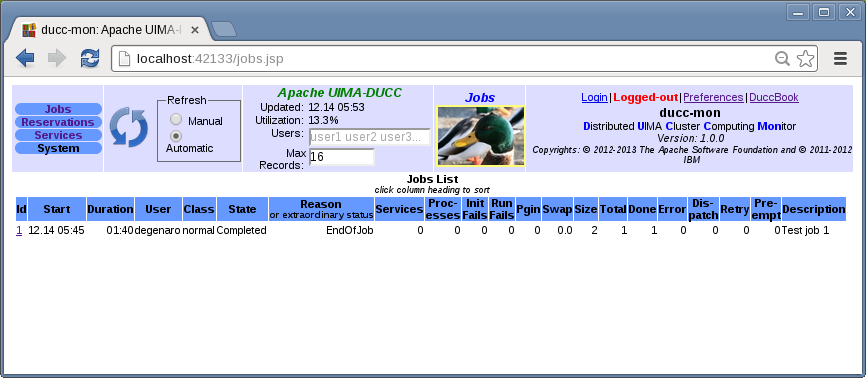
\includegraphics[width=90mm]{images/ducc-webserver/Jobs.png}
    \caption{Jobs Page}
    \end{figure}
            

      % 
% Licensed to the Apache Software Foundation (ASF) under one
% or more contributor license agreements.  See the NOTICE file
% distributed with this work for additional information
% regarding copyright ownership.  The ASF licenses this file
% to you under the Apache License, Version 2.0 (the
% "License"); you may not use this file except in compliance
% with the License.  You may obtain a copy of the License at
% 
%   http://www.apache.org/licenses/LICENSE-2.0
% 
% Unless required by applicable law or agreed to in writing,
% software distributed under the License is distributed on an
% "AS IS" BASIS, WITHOUT WARRANTIES OR CONDITIONS OF ANY
% KIND, either express or implied.  See the License for the
% specific language governing permissions and limitations
% under the License.
% 
  
    \section{Job Details Page}
    \label{sec:ws-job-details}

    This page shows details of all the processes that run in support of a job. 
    The information is divided among five tabs:
    \begin{description}
      \item[Processes] This tab contains details on all the processes for the job, both
        active, and defunct.
      \item[Work Items] This tab shows details for each individual work-item in the job.
      \item[Performance] This tab shows a performance break-down of all the UIMA analytics
        in the job.
      \item[Specification] This tab shows the job specification for the job.
      \item[Files] This tab shows the files in the log directory.
      \end{description}
      
    \subsection{Processes}
    \label{subsec:ws-processes}
    The processes page contains the following columns:
    
    \begin{description}

        \item[Id] \hfill \\
          This is the {\DUCC}-assigned numeric id of the process (not the Operating System's
          process Id). Process 0 is always the Job Driver.          

        \item[Log] \hfill \\
          This is the log name for the process. It is hyperlinked to the log itself.

        \item[Log Size] \hfill \\
          This is the size of the log in MB. If you find you have trouble viewing the log
          from the Web Server it could be because it is too big to view in the server and needs to
          be read by some other means than the Web Server.  (It is not currently paged in by 
          the Web Server, it is read in full.)

        \item[Host Name] \hfill \\
          This is the name of the host where the process ran.

        \item[PID] \hfill \\
          This is the Unix process ID (PID) of the process.

        \item[State Scheduler] \hfill \\
          % The information comes from here:
          % State Scheduler: org.apache.uima.ducc.transport.event.common.IResourceState.ResourceState

          This shows the Resource Manager state of the job. It is one of:
          \begin{description}
              \item[Allocated] - The host is currently allocated for this job by the RM.
              \item[Deallocated] - The resource manager has deallocated the shares for the job on
                this host.
          \end{description}

        \item[Reason Scheduler or extraordinary status] \hfill \\
          \phantomsection\label{itm:job-details-sched}


          % The information comes from here:
          % Reason Scheduler: org.apache.uima.ducc.transport.event.common.IResourceState.ProcessDeallocationType
          This column provides a reason for the scheduler state, when the scheduler state is other than ``Allocated''. 
          These may have ``hovers'' that provide more information
          if it is available.

            \begin{description}          
                \item[AutonomousStop] - The process terminated unexpectedly of its own accord ("crashed", or
                  simply exited.) 

                \item[Exception] - The process is terminated by the JD exception handler. 

                \item[Failed] - The process is terminated by the Agent because the JP wrapper was able to detect and 
                  communicate a fatal condition (Exception) in the pipeline.. 
                  
                \item[FailedInitialization] - The process is terminated because the UIMA initialization step failed. 
                  
                \item[Forced] - The host is preempted by RM for other work because of fair share. 
                  
                \item[JobCanceled] - The job was canceled by the user or a system administrator. 
                  
                \item[JobCompleted] - The process is canceled because of {\DUCC} restart. 
                  
                \item[JobFailure] - The job failure limit is exceeded, causing the job to be canceled by the JD.                    
                  
                \item[InitializationTimeout] - The UIMA initialization phase exceeded the configured timeout. 
                  
                \item[Killed] - The agent terminated the process for some reason. The ``Reason Agent'' field
                  should have more details in this case.
          
                \item[Stopped]	- The process was terminated by the Agent for some reason.  The hover should
                  contain more information.
                          
                \item[Voluntary] - The job is winding down, there's no more work for this host, so it stops. 
                  
                \item[Unknown] - None of the above. This is an exceptional condition, sometimes an
                  internal {\DUCC} error. Check the JP and JD logs for possible causes..
            \end{description}

          \item[State Agent] \hfill \\
          \phantomsection\label{itm:job-details-state}

          % This state comes from here:
          % State Agent: org.apache.uima.ducc.transport.event.common.IProcessState.ProcessState
            This shows the {\DUCC} Agent's view of the state of the process.
            \begin{description}
               \item[Starting] The {\DUCC} process manager as issued a request to the assigned {\DUCC} Agent to
                 start the process.
               \item[Initializing] The process is initializing.  Usually this means the UIMA analytic
                 pipeline (Job Process) is executing its initialization method.
              \item[Running] The Job Process has completed the initialization phase and is ready for 
                or actively executing work.
              \item[Stopped] The {\DUCC} Agent reports the process is stopped and (and has exited).
              \item[Failed] The {\DUCC} Agent reports the process failed with errors.  This usually
                means that UIMA-AS has detected exceptions in the pipeline and reported them
                to the Job Driver for logging.
              \item[FailedInitialization] The process died during the UIMA initialization phase.
              \item[InitializationTimeout] The process exceeded the site's limit for time spent
                in UIMA initialization.
              \item[Killed] The {\DUCC} Agent killed the process for some reason.  There are
                three reasons for this:
                \begin{enumerate}
                  \item The Job Processes failed to initialize,
                  \item The Job Process timed out during initialization,
                  \item The process exceeded its allowed swap.
                \end{enumerate}
              \item[Abandoned] It is possible to cancel a specific process of a job.  Usually
                this is because it became ``stuck'' because of hardware failure.  If a process
                is killed in \hyperref[sec:cli.ducc-cancel]{this way}, the state is recorded as {\em Abandoned}.
            \end{description}
            
          \item[Reason Agent] \hfill \\
          \phantomsection\label{itm:job-details-agent}

          This shows extended reason information if a process exited other than having run out
          of work to do.

            \begin{description}
              \item[AgentTimedOutWatingForORState] The {\DUCC} Agent is expecting a state update
                from the {\DUCC} Orchestrator.  Timer on this wait has expired.  This usually 
                indicates an infrastructure or communication problem.
              \item[Croaked] The process exited for no good or clear reason, it simply vanished.
              \item[Discontinued] This is the normal reason when the process is stopped as directed.
              \item[ExceededShareSize] The process exceeded it's declared memory size.
              \item[ExceededSwapThreshold] The process exceeded the configured swap threshold.
              \item[FailedInitialization] The process was terminated because the UIMA 
                initialization step failed.
              \item[InitializationTimeout] The process was terminated because the UIMA initialization
                step took too long.
              \item[JPHasNoActiveJob] This is set when an agent looses connectivity while its
                JPs are running. The job finishes (stopped or killed). The agent regains
                connectivity. The OR publish no longer includes the job but the agent still has
                processes running for that job. The agent kills ghost processes with the reason:
                JPHasNoActiveJob.
              \item[LowSwapSpace] The process was terminated because the system is about to run
                out of swap space.  This is a preemptive measure taken by {\DUCC} to avoid exhaustion
                of swap, to effect orderly eviction of the job before the operating system starts
                its own reaping procedures.
              \item[AdministratorInitiated] The process was canceled by an administrator.
              \item[UserInitated] The process was canceled by the owning user.
            \end{description}
                    
          \item[Exit] \hfill \\
            The process exit code or signal.
            
          \item[Time Init] \hfill \\
            This is the clock time this process spent in initialization.
            
          \item[Time Run] \hfill \\
            This is the clock time this process spent in executing, not including
            initialization.
            
          \item[Time GC] \hfill \\
            This is amount of time spent in Java Garbage Collection for the process.
            
          \item[PgIn] \hfill \\
            This is the number of page-in events on behalf of the process.

          \item[Swap] \hfill \\
            This is the amount of swap space on the machine being consumed by the process.

          \item[\%CPU] \hfill \\
            Current CPU percent consumed by the process.  This will be $>$ 100\% on 
            multi-core systems if more than one core is being used.  Each core contributes
            up to 100\% CPU, so, for example, on a 16-core machine, this can be as high
            as 1600\%.
            
          \item[RSS] \hfill \\
            The amount of real memory being consumed by the process (Resident Storage Size)
            
          \item[Time Avg] \hfill \\
            This is the average time in seconds spent per work item in the process.
            
          \item[Time Max] \hfill \\
            This is the maximum time in seconds spent per work item in the process.
            
          \item[Time Min] \hfill \\
            This is the minimum time in seconds spent per work item in the process.
            
          \item[Done] \hfill \\
            This is the number of work items processed in this process.
            
          \item[Error] \hfill \\
            This is the number of exceptions processing work items in this process.
                      
          \item[Dispatch] \hfill \\
            The number of work items currently dispatched.
              
          \item[Retry] \hfill \\
            This is the number of work items that were retried in this process for any reason, excluding
            preemption.
            
          \item[Preempt] \hfill \\
            This is the number of work items that were preempted from this process, if
            fair-share caused preemption.
            
          \item[JConsole URL] \hfill \\
            This is a URL that can be used to connect via JMX to the processes, e.g. via
            jconsole.

      \end{description}
      
    \begin{figure}[ht!]
    \centering
    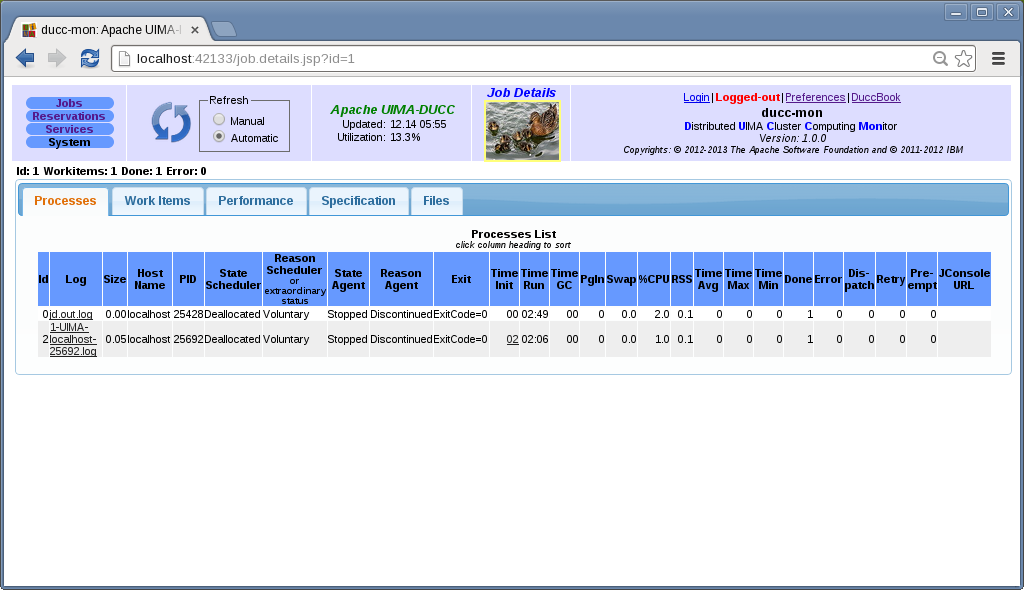
\includegraphics[width=90mm]{images/ducc-webserver/Job-Details-Processes.png}
    \caption{Processes Tab}
    \end{figure}
    
   \subsection{Work Items}
   \label{subsec:ws-work-items}
   This tab provides details for each individual work item.  Columns include:

   % The data comes from here: org.apache.uima.ducc.common.jd.files.IWorkItemState.State    
   \begin{description}
     \item[SeqNo]  \hfill \\
       This is the sequence work items are fetched from the Collection Reader's
       getNext() method by the {\DUCC} Job Driver.
     \item[Id]  \hfill \\
       This is the name of the work item.
     \item[Status]  \hfill \\
       The is the current state of the work item.  
       States include:
       \begin{description}
         \item[ended] The work item is complete.
         \item[error] The work item ended with errors.
         \item[operating] The work item is current being executed.
         \item[retry] The work item is being retried.
         \item[start] The work item has been picked up for execution and {\DUCC} is waiting
           for confirmation that it is running.
       \end{description}
       If a work item has not yet been retrieved from the Collect Reader it does not show
       on this page.
     \item[Delivery Time (sec)]  \hfill \\
       The time spent in getting a work item from the Job Driver to a Job Process.
     \item[Process Time (sec)]  \hfill \\
       The time spent processing the work item.
     \item[Investment Time (sec)]  \hfill \\
       The time spent processing the work item during the current epoch.
     \item[Node (IP)]  \hfill \\
       The host IP where the work item was processed.
     \item[Node (Name)]  \hfill \\
       The host name where the work item was processed.
     \item[PID]  \hfill \\
       The Unix Process Id that the work item was processed in.
   \end{description}
    
    \begin{figure}[ht!]
    \centering
    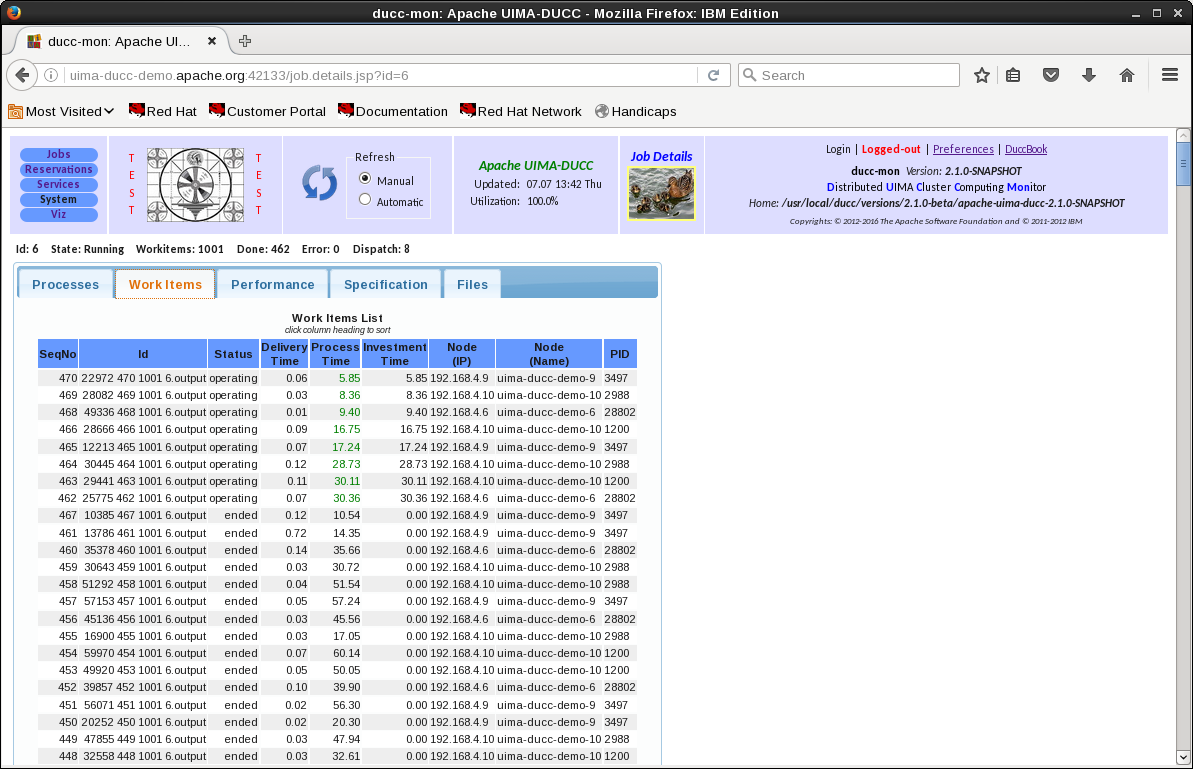
\includegraphics[width=90mm]{images/ducc-webserver/Job-Details-WorkItems.png}
    \caption{Work Items Tab}
    \end{figure}  

   \subsection{Performance}
   \label{subsec:performance}
   This tab shows performance summaries of all the pipeline components.  The statistics
   are aggregated over all instances of each component in each process of the job.
   
   \begin{description}
     \item[Name]  \hfill \\
       The short name of the analytic.
     \item[Total]  \hfill \\
       This is the total time in days, hours, minutes, and seconds taken by each
       component of the pipeline.
     \item[\% of Total]  \hfill \\
       This is the percent of the total usage consumed by this analytic.
     \item[Avg]  \hfill \\
       This is the average time spent by all the instances of the analytic.
     \item[Min]  \hfill \\
       This is the minimum time spent by any instance of the analytic.
     \item[Max]  \hfill \\
       This is the maximum time spent by any instance of the analytic.
   \end{description}
    
    \begin{figure}[ht!]
    \centering
    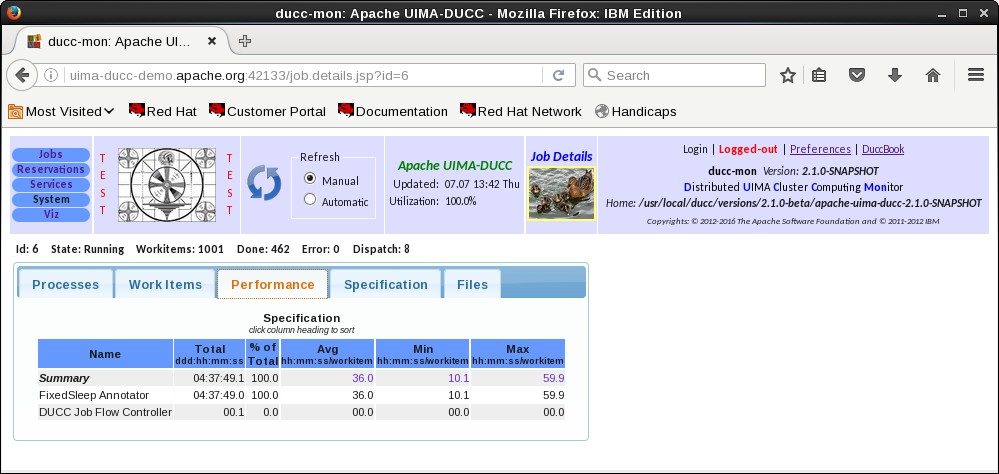
\includegraphics[width=90mm]{images/ducc-webserver/Job-Details-Performance.png}
    \caption{Performance Tab}
    \end{figure}  
       
   \subsection{Specification}
   This tab shows the full job specification in the form of a Java Properties
   file.  This will include all the parameters specified by the user, plus those
   filled in by {\DUCC}.
    
    \begin{figure}[ht!]
    \centering
    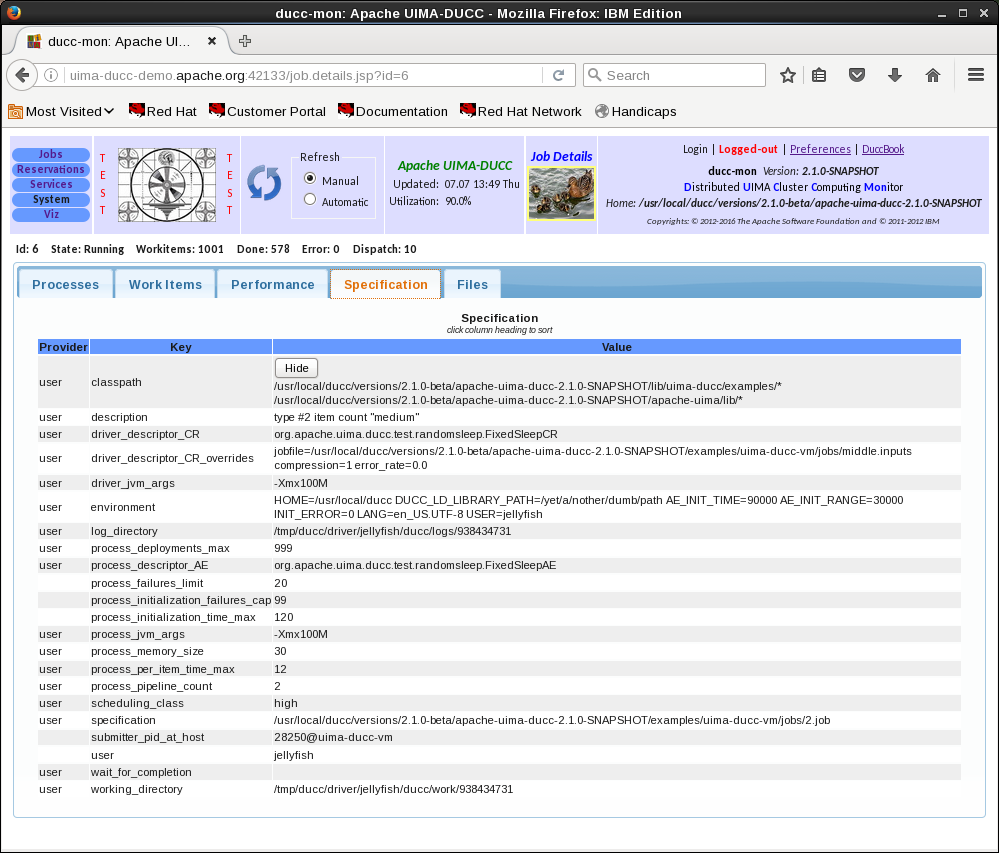
\includegraphics[width=90mm]{images/ducc-webserver/Job-Details-Specification.png}
    \caption{Specification Tab}
    \end{figure}  
    
   \subsection{Files}
   This tab shows the files in the log directory.

      % 
% Licensed to the Apache Software Foundation (ASF) under one
% or more contributor license agreements.  See the NOTICE file
% distributed with this work for additional information
% regarding copyright ownership.  The ASF licenses this file
% to you under the Apache License, Version 2.0 (the
% "License"); you may not use this file except in compliance
% with the License.  You may obtain a copy of the License at
% 
%   http://www.apache.org/licenses/LICENSE-2.0
% 
% Unless required by applicable law or agreed to in writing,
% software distributed under the License is distributed on an
% "AS IS" BASIS, WITHOUT WARRANTIES OR CONDITIONS OF ANY
% KIND, either express or implied.  See the License for the
% specific language governing permissions and limitations
% under the License.
% 

\section{Reservations Page}
\label{sec:ws-reservations}

This page shows details of all reservations.  There are two types of reservations: {\em managed}
and {\em unmanaged}.

A {\em managed reservation} is a reservation whose process is fully managed by {\DUCC}.  This process
is any arbitrary process and is submitted with the
\hyperref[sec:cli.ducc-process-submit]{ducc\_process\_submit} CLI.  The lifetime of the reservation
starts at the time {\DUCC} assigns a unique ID, and ends when the process terminates for any reason.

An {\em unmanaged reservation} is essentially a sandbox for the user.  {\DUCC} starts no processes
in the reservation and manages none of the processes which run on that host.  The lifetime of the
reservation starts at the time {\DUCC} assigns a unique ID, and ends when the submitter or system
administrator cancels it.

The Reservations page contains the following columns: 
\begin{description}

\item[Id] \hfill \\
  This is the unique {\DUCC} numeric id of the reservation as assigned when the reservation is made.
  If this is a {\em managed} reservation, the ID is hyperlinked to a
  \hyperref[sec:ws-managed-reservation-details]{Managed Reservation Details} page with extended
  details on the process running in the reservation.

\item[Start] \hfill \\
  This is the time the reservation was made.
  
\item[Duration] \hfill \\
  A time in green is the length of time the active reservation has been assigned.  
  A time in black is the length of time the completed reservation was assigned. 
  
\item[User] \hfill \\
  This is the userid that made the reservation.
  
\item[Class] \hfill \\
  This is the scheduling class used to schedule the reservation.
  
\item[Type] \hfill \\
  This is the reservation type, {\em managed} or {\em unmanaged}, as described 
  \hyperref[sec:ws-reservations]{above}.

\item[State] \hfill \\
  % 1. org.apache.uima.ducc.transport.event.common.IDuccState
  This is the status of the reservation. Values include: Received - Reservation
  has been vetted, persisted, and assigned unique Id.
  \begin{description}
  \item[Assigned] - The reservation is active. 
  \item[Completed] - The reservation has been terminated.
  \item[Received] - The Reservation has been vetted, persisted, and assigned a unique ID.
  \item[WaitingForResources] - The reservation is waiting for the Resource Manager to find and 
    schedule resources. 
  \end{description}

\item[Reason] \hfill \\

  % 2. org.apache.uima.ducc.transport.event.common.IDuccCompletionType

  If a reservation is not active, this shows the reason.  Note that for
  {\em unmanaged reservations}, even if the user has processes running in the
  reservation, {\DUCC} does NOT attempt to terminate those processes (hence, ``unmanaged''.)

  For {\em managed reservations}, {\DUCC} does terminate the associated process.

  \begin{description}
  \item[CanceledBySystem] - In the case of the special JobDriver reservation, this is
    canceled by {\DUCC} and reestablished on reboot; hence the state is a result of {\DUCC}
    having been restarted.

    In all other cases, it is a result of {\DUCC} being restarted {\em COLD}.  When
    {\DUCC} is started {\em COLD}, all previous reservations are canceled.  (When {\DUCC}
    is started {\em WARM}, the default, previous reservations are preserved.)
  \item[CanceledByAdmin] - The {\DUCC} administrator released the reservation. 
  \item[CanceledByUser] - The reservation owner released the reservation. 
  \item[ResourcesUnavailable] - The Resource Manager was unable to find free or freeable resources 
    to match the resource request. 
  \item[ProgramExit] - The reservation is a {\em managed} reservation and the associated
    process has exited.
  \end{description}

\item[User Processes] This is the number of processes owned by the user running in the reservation.  
  
  Note that even for {\em unmanaged} reservations, the {\DUCC} agent tracks processes owned
  by the user and reports on them.  This allows better identification and management of
  abandoned reservations.
          
\item[PgIn] This is the number of page-in events for the managed reservation.

\item[Swap] This is the total swap space for the managed reservation.

\item[Memory] \hfill \\
  The memory size in GB of the reservation.  This is the amount of memory that
  was {\em requested}.  In the case of RESERVE policy reservations, that actual memory
  of the reserved machine may be greater.
  
\item[Host Names] \hfill \\
  The host names of the machines where the resources are allocated.
  
\item[Description] \hfill \\
  This is the description string from the --description string from submit.
\end{description}

    \begin{figure}[ht!]
    \centering
    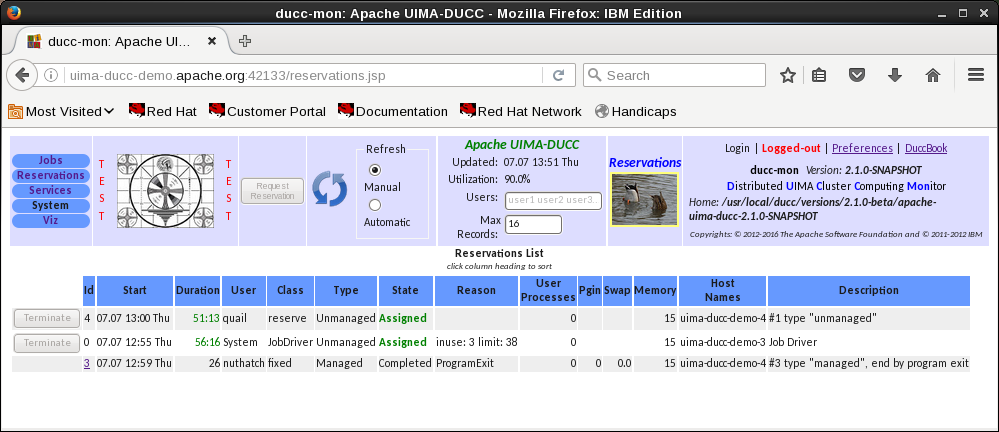
\includegraphics[width=90mm]{images/ducc-webserver/Reservations.png}
    \caption{Reservations Page}
    \end{figure}

